\section{Experiments}
\label{sec:exp}
\subsection{Datasets}
To evaluate our model's performance and generalization, a diverse suite of seven public hyperspectral datasets are conducted, covering \textit{indoor, outdoor, and remote sensing} scenarios. Information of dataset are summarized in Tab.~\ref{tab:dataset_details}.

Our setup deliberately embraces heterogeneity, with spectral bands ranging from 31 (CAVE) to 191 (Washington DC), and substantially differing spatial resolutions and spectral ranges from sensors like ROSIS and Hyperion. This diversity provides the perfect testbed for validating the spectral agnosticism of our SSA framework. We followed standard train/test splits for each dataset, using appropriate patch sizes as detailed in the table.
% \subsubsection{Evaluation Metrics}
\subsection{Implementation Details} 
Our SSA model and all experiments were implemented using the PyTorch framework~\cite{NEURIPS2019_9015}. 
All training and inference were conducted on a single NVIDIA RTX 4090 GPU.
For the training process, we use the AdamW optimizer~\cite{loshchilov2017decoupled} and trained the model for 2000 epochs with a batch size of 4. The learning rate was managed by a cosine annealing learning rate scheduler, starting from 2e-4 and annealing to 1e-5. To enable the spectral agnosticism of MK, the crucial hyperparameter for the maximum channel, $C_{\max}$, was set to 194. Both encoders are based on the EDSR architecture~\cite{lim2017enhanced}.

\begin{figure*}
    \centering
    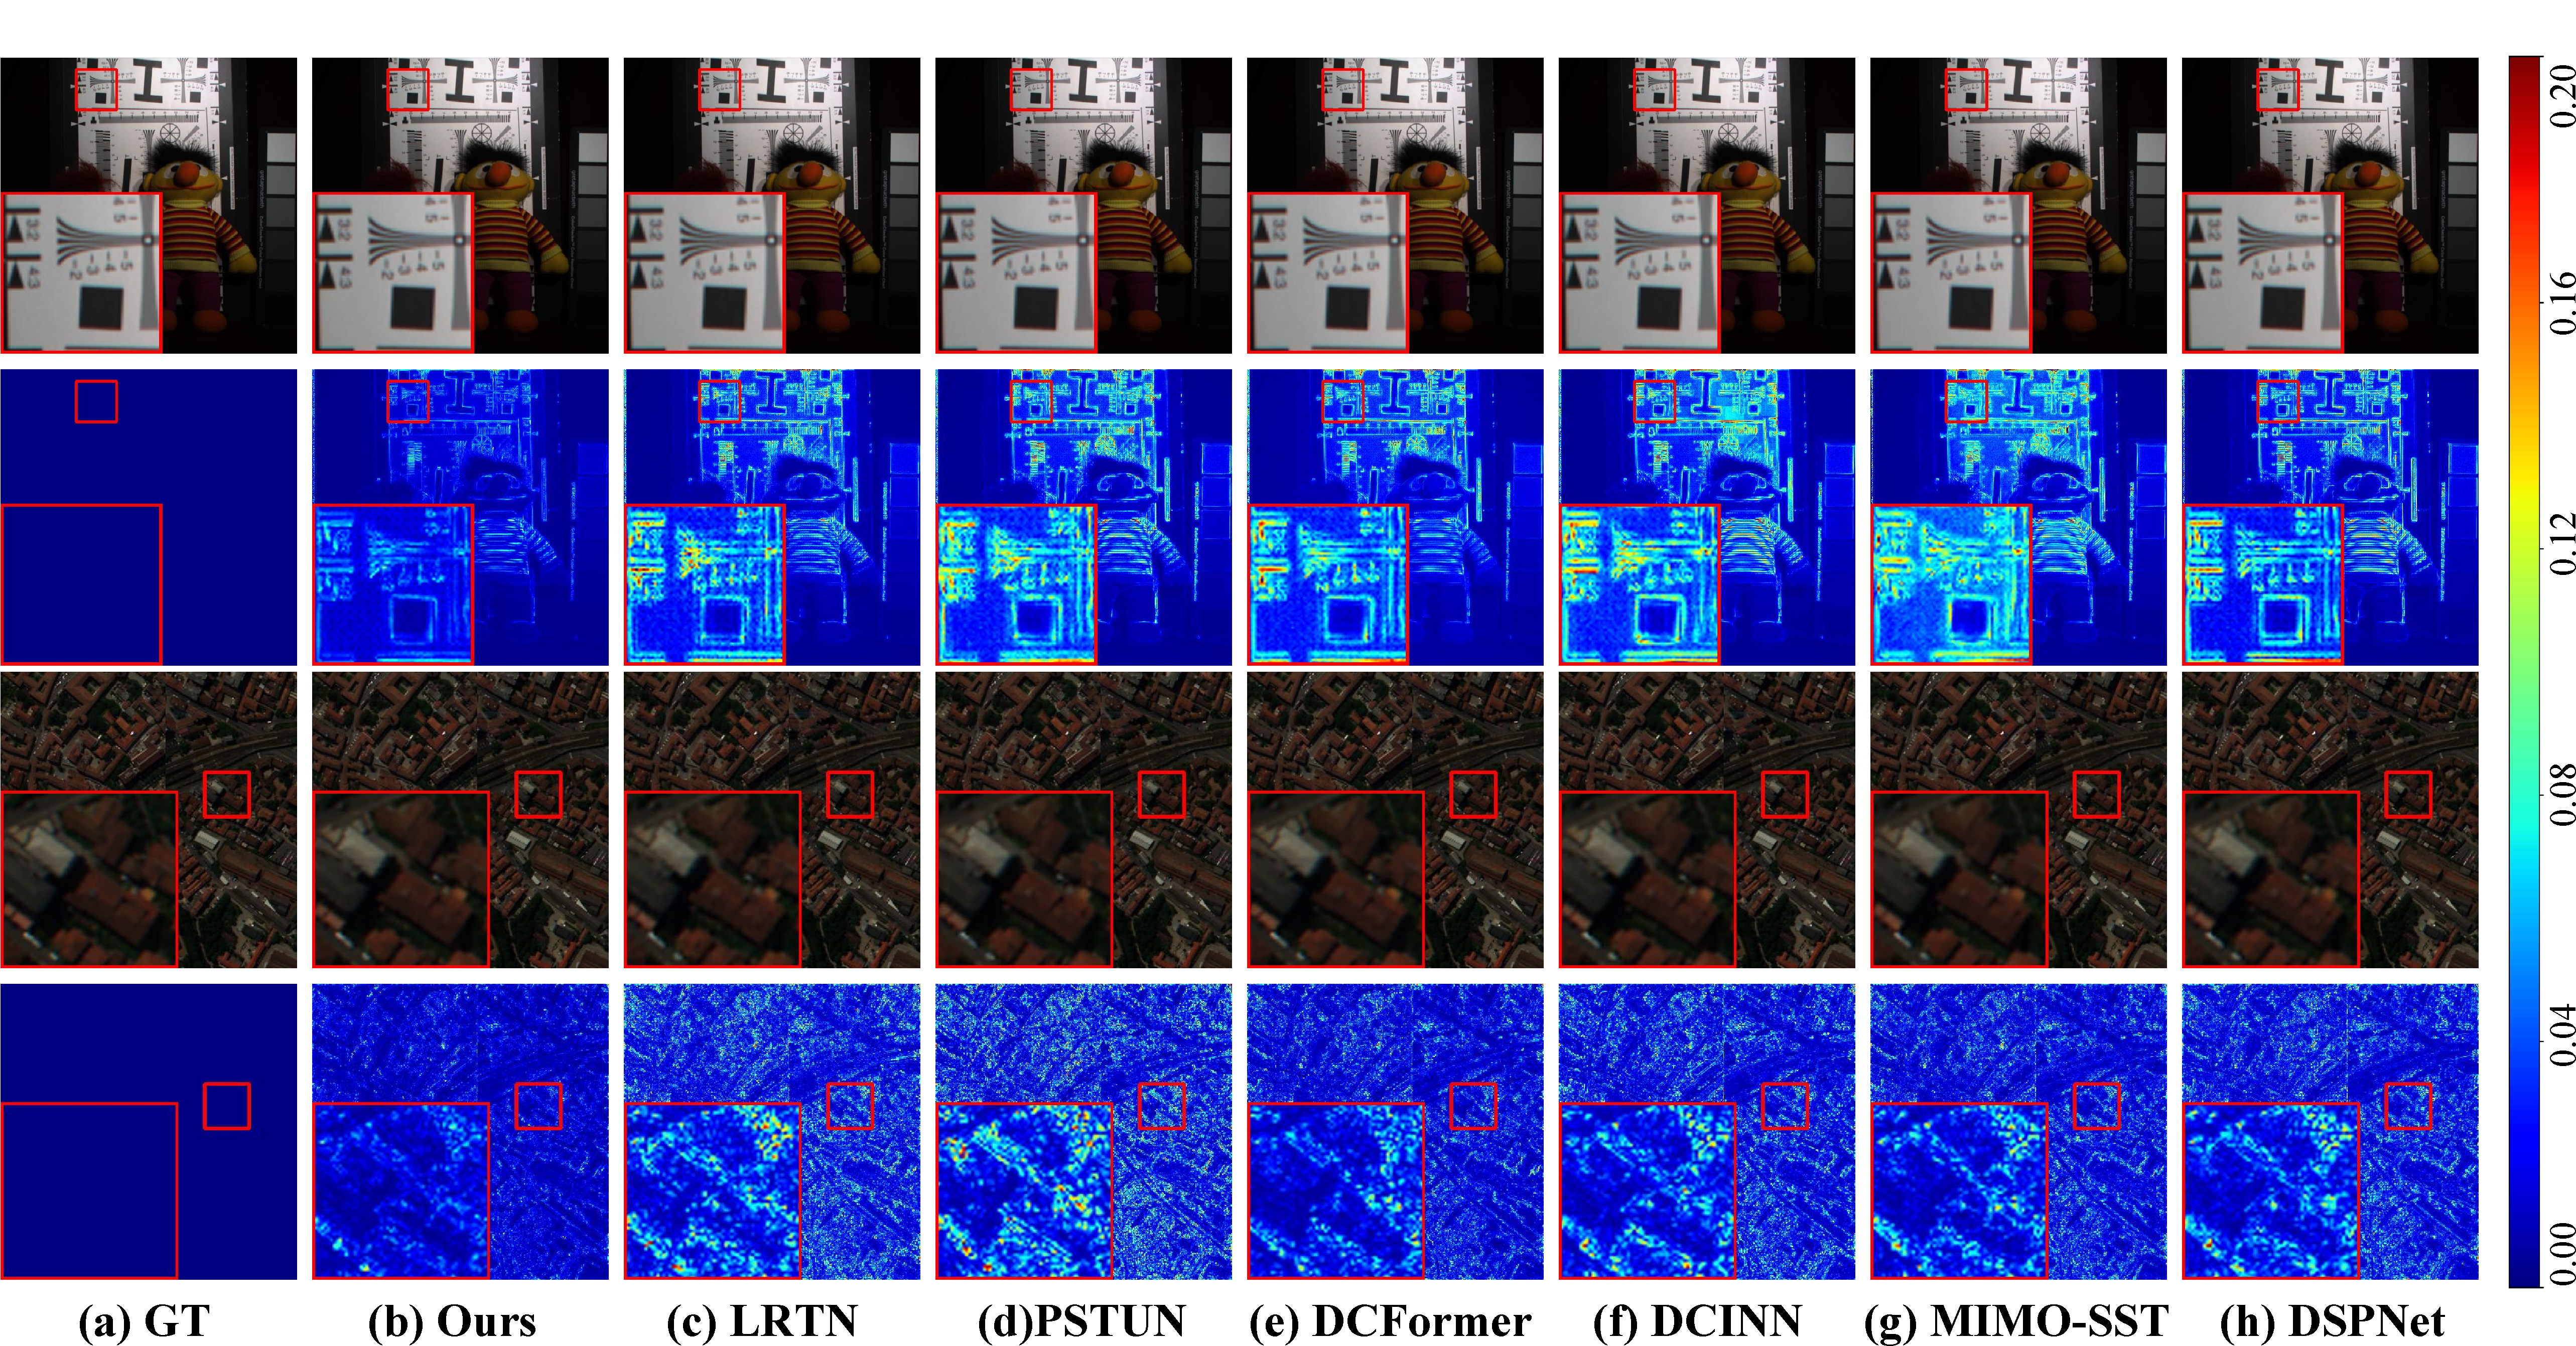
\includegraphics[width=0.90\textwidth]{Figs/hsi.pdf}
    \caption{The upper and lower parts respectively showcase the fused images and error maps from the CAVE and PaviaC datasets. Red rectangles depict some close-up shots.}
    \label{fig:hsi}
\end{figure*}
\subsection{Main Results}
To highlight the fundamental difference between our proposed model and existing methods, for each dataset (at a $4 \times$ ratio), we trained a dedicated model independently for all SOTA methods to be compared, and evaluated them on the test sets with ratios of $4 \times$, $8 \times$, $16 \times$, and $32 \times$. For our method, we trained only a single, unified model, with the training set composed of a mixture of training samples from the seven datasets. The evaluation on the test set was conducted in the same manner as before. Additionally, we adopted four widely used quality metrics, namely Peak Signal-to-Noise Ratio (PSNR), Spectral Angle Mapper (SAM), Erreur Relative Globale Adimensionnelle de Synthèse (ERGAS), and the Structural Similarity (SSIM). The calculation formulas for the above indicators can be found in the App.\S~\ref{QualityIndexes}.
\subsubsection{Quantitative Comparison}
Tab.~\ref{tab:cave_pavia_quantitative_comparison} presents the quantitative comparison of all methods on the CAVE and PaviaC datasets, under both in-distribution (the $\times4$ training scale) and out-of-distribution ($\times8$, $\times16$, and $\times32$ scales) settings. The data in the table indicates that our method achieves SOTA performance across all in-distribution metrics. In the out-of-distribution evaluation, our model secures the best or second-best results on nearly all out-of-distribution metrics. Although methods like DCFormer~\cite{wu2025fully}, DSPNet~\cite{sun2023dual}, and PSTUN~\cite{wang2025perceptive} also achieve strong second-best results in some specific cases, they suffer from the inability to handle all scales and exhibit inconsistent performance. The quantitative comparison results for the other five datasets can be found in App.\S~\ref{sec:add_res}.
To provide a comprehensive view of the performance across all datasets, we plot the PSNR metrics of all methods in a line chart (see Fig.~\ref{fig:psnr}). It can be observed that our model does not compromise on reconstruction quality; its performance can even surpass that of specialized models that were individually trained for each specific dataset. Our method provides the best in-distribution accuracy and demonstrates robust generalization to unseen scales.
 \begin{table}[!t]
    \centering
    \caption{Ablation study of MK on the PaviaC dataset (See \S\ref{ablation:necess-nk}).}
    % Our jointly trained model with MK achieves performance on par with a hyper-specialized variant trained individually for the dataset.}
    \label{tab:ablation_mk}
    \resizebox{\columnwidth}{!}{%
    \begin{tabular}{l|c|cccc}
        \toprule
        \multicolumn{2}{c|}{\textbf{Model}} & \textbf{PSNR}($\uparrow$) & \textbf{SAM}($\downarrow$) & \textbf{ERGAS}($\downarrow$) & \textbf{SSIM}($\uparrow$) \\
        \midrule
        \multirow{2}{*}{$\times 4$} &w/o MK & 45.85 $\pm$ 1.80 & \textbf{2.01 $\pm$ 0.29} & \textbf{1.06 $\pm$ 0.11} & 0.995 $\pm$ 0.001 \\
                                         & \textbf{Ours} & \textbf{45.92 $\pm$ 1.75} & 2.02 $\pm$ 0.30 & 1.07 $\pm$ 0.11 & \textbf{0.996 $\pm$ 0.000} \\
        \hline
        \multirow{2}{*}{$\times 8$} &w/o MK & \textbf{38.62 $\pm$ 0.65} & 4.75 $\pm$ 0.07 & 3.49 $\pm$ 0.06 & 0.959 $\pm$ 0.004 \\
                                         & \textbf{Ours} & 38.59 $\pm$ 0.67 & \textbf{4.74 $\pm$ 0.06} & \textbf{3.47 $\pm$ 0.05} & \textbf{0.960 $\pm$ 0.004} \\
        \hline
        \multirow{2}{*}{$\times 16$} &w/o MK & 34.95 $\pm$ 0.03 & 6.92 $\pm$ 0.08 & 5.18 $\pm$ 0.07 & \textbf{0.936 $\pm$ 0.002} \\
                                         & \textbf{Ours} & \textbf{35.00 $\pm$ 0.02} & \textbf{6.89 $\pm$ 0.08} & \textbf{5.16 $\pm$ 0.07} & 0.935 $\pm$ 0.002 \\
        \hline
        \multirow{2}{*}{$\times 32$} &w/o MK & \textbf{32.81 $\pm$ 0.25} & 8.51 $\pm$ 0.20 & 6.25 $\pm$ 0.29 & 0.921 $\pm$ 0.001 \\
                                         & \textbf{Ours} & 32.79 $\pm$ 0.26 & \textbf{8.49 $\pm$ 0.19} & \textbf{6.24 $\pm$ 0.30} & \textbf{0.922 $\pm$ 0.001} \\
        \bottomrule
    \end{tabular}%
    }
\end{table}
\subsubsection{Qualitative Comparison}
To illustrate the advantages of our method, we provide a visual comparison in Fig.~\ref{fig:hsi} with SOTA approaches, including close-ups and error maps to highlight specific details. Visually, the results generated by our SSA model are markedly superior and most faithful to the GT. 
Visually, our SSA model yields results most faithful to the ground truth. The close-up views reveal that our method effectively recovers fine details, such as the texture of the stuffed toy and crisp lines on the chart, while competitors often suffer from blurriness and artifacts. Similarly, it reconstructs clearer architectural structures in the remote sensing scene. This superiority is corroborated by the error maps: while ours remain predominantly dark blue (indicating minimal residuals), SOTA methods display significant high-energy areas (yellow/red) along object boundaries, demonstrating the robust accuracy of our unified approach.
% To illustrate the advantages of our method, we provide a visual comparison in Fig.~\ref{fig:hsi} with six deep learning methods, including close-ups and error maps to highlight specific details. In the close-up images of ``\textit{Chart and Stuffed Toy}'' and ``\textit{ara2}'', our fusion results closely match the ground truth, achieving the highest quality. When comparing the error maps, where colors closer to blue indicate higher accuracy and colors closer to red indicate greater error, it is clear that SSA excels in detail recovery compared to other methods, whether on real outdoor remote sensing datasets or indoor hyperspectral datasets. 
\subsection{Ablation Studies}
\label{sec:ablation}
% --- Transposed Table Starts Here ---


\begin{table}[!ht]
\centering
\caption{
\textbf{Generalization to Unseen Bands and Fractional Scales.}
Top: generalization on unseen datasets at $\times4$ scale, including Houston and Loukia.
Bottom: generalization on unseen scales on CAVE (trained at $\times4$ ratio).
Results of DCFormer/PSTUN/LRTN are obtained by bicubic resizing based on $\times 4$ ratio.
}
\label{tab:generalization_fractional_unseen}
\resizebox{0.95\linewidth}{!}{%
\begin{tabular}{lcccc}
\toprule
\textbf{Model} & \textbf{PSNR($\uparrow$)} & \textbf{SAM($\downarrow$)} & \textbf{ERGAS($\downarrow$)} & \textbf{SSIM($\uparrow$)} \\
\midrule

\multicolumn{5}{c}{\textit{Unseen Dataset — Houston (48 bands, $\times4$ scale)}} \\
\midrule
DCFormer & 38.55 & 3.21 & 4.09 & 0.972 \\
PSTUN & 38.52 & 3.15 & 3.98 & 0.975 \\
LRTN & 38.65 & 3.12 & 3.91 & \textbf{0.980} \\
\textbf{Ours} & \textbf{38.71} & \textbf{3.09} & \textbf{3.85} & 0.978 \\
\midrule

\multicolumn{5}{c}{\textit{Unseen Dataset — Loukia (176 bands, $\times4$ scale)}} \\
\midrule
DCFormer & 36.25 & \textbf{3.88} & 3.65 & 0.958 \\
PSTUN & 35.80 & 4.12 & 3.82 & 0.952 \\
LRTN & 35.92 & 4.05 & 3.78 & 0.955 \\
\textbf{Ours} & \textbf{36.42} & 3.95 & \textbf{3.55} & \textbf{0.962} \\
\midrule

\multicolumn{5}{c}{\textit{Fractional Scales — CAVE (trained only at $\times4$) $\times3.2$ scale}} \\
\midrule
Bicubic & 38.50 & 5.12 & 4.85 & 0.945 \\
DCFormer & 44.65 & \textbf{2.45} & 1.95 & 0.990 \\
PSTUN & 43.90 & 2.62 & 2.25 & 0.985 \\
LRTN & 44.35 & 2.58 & 2.08 & 0.988 \\
\textbf{Ours (direct)} & \textbf{45.02} & 2.48 & \textbf{1.81} & \textbf{0.993} \\
\midrule

\multicolumn{5}{c}{\textit{Fractional Scales — CAVE (trained only at $\times4$) $\times5.7$ scale}} \\
\midrule
Bicubic & 32.20 & 6.85 & 6.10 & 0.895 \\
DCFormer & 42.95 & 3.02 & 2.45 & 0.984 \\
PSTUN & 41.25 & 3.25 & 2.72 & 0.980 \\
LRTN & 42.80 & \textbf{2.88} & 2.55 & 0.982 \\
\textbf{Ours (direct)} & \textbf{43.49} & 2.91 & \textbf{2.17} & \textbf{0.991} \\
\bottomrule
\end{tabular}}
\end{table}


\subsubsection{The Necessity of Matryoshka Kernels}
\label{ablation:necess-nk}
% --- Transposed Table Ends Here ---
To validate the role of MK, we validated an w/o MK variant by replacing our MKLs with standard fixed-channel convolutions and trained it independently on each dataset.

Tab.~\ref{tab:ablation_mk} compares this individually trained variant against our single, jointly trained model. The results show that the performance between the two models is highly comparable across all scales. While the `w/o MK' variant occasionally performs marginally better, our unified model with MK often matches or exceeds its performance.
This demonstrates that our model, achieves performance that is on par with specialized models. \\
% For further analysis, we provide more ablation studies in Suppl.\,\S 1.3, which investigates the model's generalization to unseen bands and fractional scales.
\subsubsection{Unseen Bands and Fractional Scales}
\label{sec:generalization}
We further evaluate the generalization of our pretrained model under two challenging settings: unseen datasets with different spectral bands and unseen fractional scales.

\textbf{Unseen datasets (unseen bands).}
We first test on two datasets whose spectral configurations are not observed during training: Houston with 48 bands and Loukia with 176 bands, both evaluated at the $\times4$ scale.
As shown in Tab.~\ref{tab:generalization_fractional_unseen}, our method, finetuned for only 500 iterations, consistently achieves top-tier performance across metrics.
On Houston, our model obtains the best PSNR/SAM/ERGAS (38.71\,dB / 3.09 / 3.85) and remains competitive in SSIM (0.978), demonstrating robust generalization to a different band setup.
On Loukia, our method again delivers the best reconstruction quality, achieving the highest PSNR (36.42\,dB), the lowest ERGAS (3.55), and the highest SSIM (0.962), while remaining competitive in SAM.
These results indicate that our learned spectral representation transfers well across datasets with varying band numbers and distributions.

\textbf{Unseen fractional scales.}
We further evaluate scale generalization by testing on CAVE at fractional scales $\times3.2$ and $\times5.7$, while training is performed only at the integer scale $\times4$.
For methods without native continuous scaling, we follow a strong baseline protocol: generate the $\times4$ output and then resize to the target fractional scale via Bicubic interpolation ($\times4\!\to$Bicubic).
Tab.~\ref{tab:generalization_fractional_unseen} shows that our method directly predicts fractional scales and achieves the best PSNR at both scales (45.02\,dB at $\times3.2$ and 43.49\,dB at $\times5.7$), together with the lowest ERGAS (1.81 and 2.17) and the highest SSIM (0.993 and 0.991).
Overall, these results confirm that our continuous representation provides genuine scale-agnostic capability, generalizing effectively beyond the discrete scale seen during training and outperforming strong $\times4\!\to$Bicubic baselines.

\subsubsection{Analysis of Learned Kernel Structures}
\begin{figure}[!t]
    \centering
    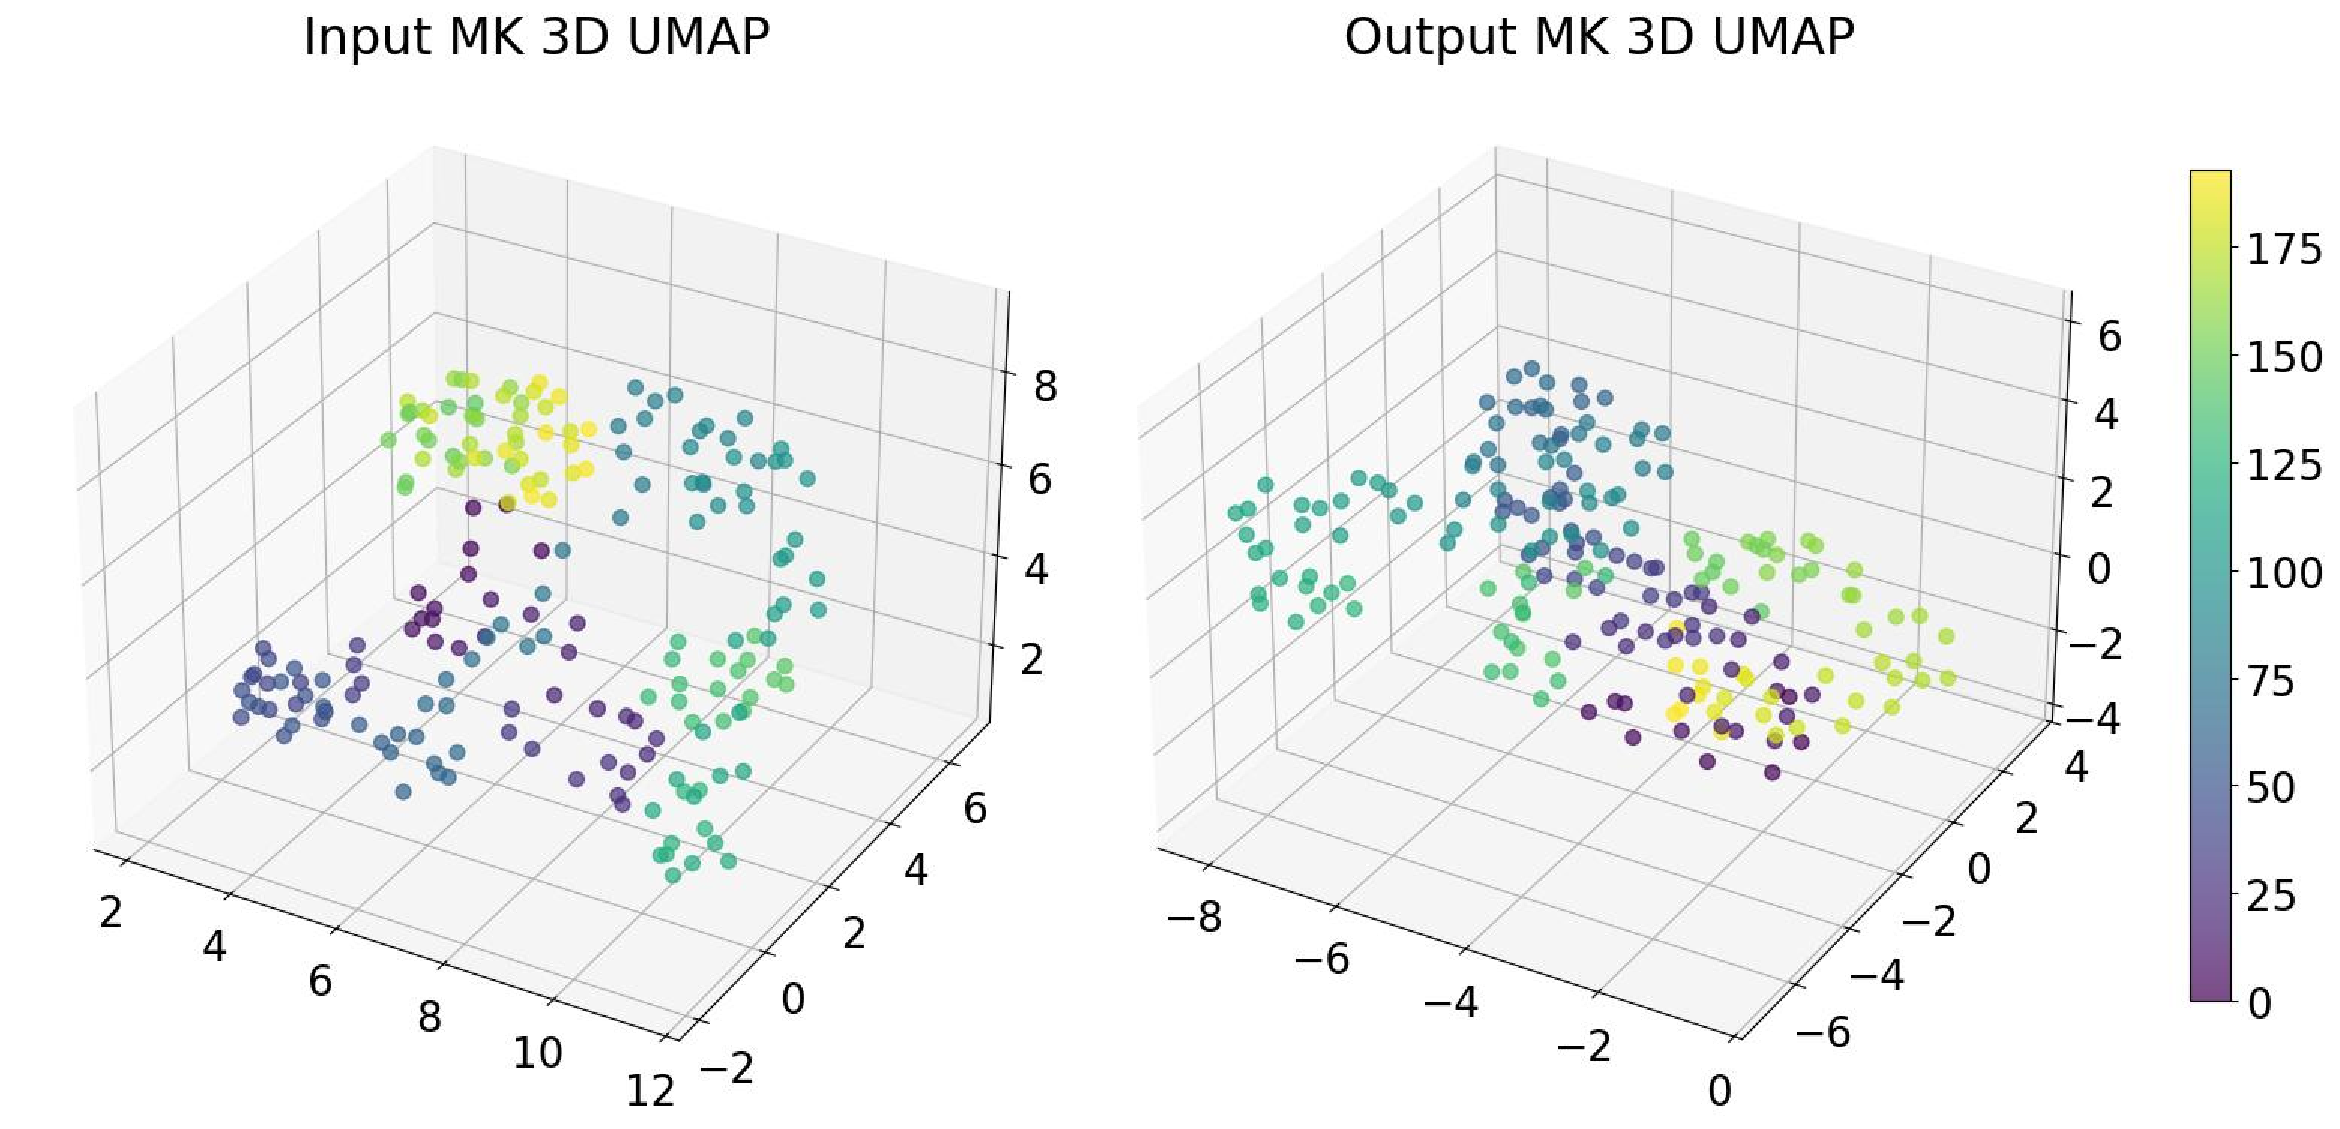
\includegraphics[width=1\linewidth]{Figs/mkumap.pdf}
    \caption{%Learned Structures of Input and Output Matryoshka Kernels.
     UMAP~\cite{mcinnes2018umap} visualization of the learned MK weights, which form a smooth manifold that reveals the model's encoding of spectral continuity, key to its generalization.}
    \label{fig:umap}
\end{figure}
To investigate the internal working mechanisms of our MKs, we visualized the weight structures of both the input and output kernels using UMAP~\cite{mcinnes2018umap}, as shown in Fig.~\ref{fig:umap}. Each point in the visualizations corresponds to a spectral channel, colored by its index. 
As can be seen, the projected points form smooth and continuous manifolds rather than a randomly scattered cloud. This indicates that the learning process of the kernels has formed a meaningful, layered manifold structure, where the network actively captures the high correlation between adjacent spectral bands. 
This learned internal structure is key to our model's ability to generalize effectively across different sensors.

\subsection{Efficiency Analysis}
We conducted efficiency analyses on all the comparison models and ablation experiments on our model scaling, which are detailed in App.\S~\ref{effana} and App.\S~\ref{modelscaling}.
